% No-photos sign for the poster footer (built to assets/no_photos.pdf by make): a line-art camera under a prohibition ring,
% ISO 7010 P029 layout (bar from upper left to lower right), drawn flat and thin. 24 x 24 mm, vector, no text.
% Build: make assets/no_photos.pdf (pdflatex)
\documentclass[tikz,border=0pt]{standalone}
\usetikzlibrary{calc}
\definecolor{ink}{HTML}{1A1A1A}
\definecolor{stop}{HTML}{E30613}   % process red (CMYK 0/100/100/0), prints as a clean signal red
\begin{document}
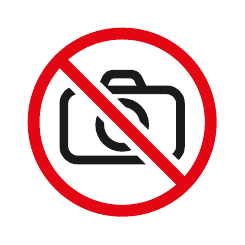
\begin{tikzpicture}[x=1mm, y=1mm, line cap=round, line join=round]
  \def\w{1.5}            % ring and bar width (mm)
  \def\R{11.25}          % ring centre-line radius: outer edge at 12 mm
  \useasboundingbox (0,0) rectangle (24,24);   % TikZ ignores line width; keep the ring's outer edge inside
  % camera: body, viewfinder hump, lens
  \begin{scope}[ink, line width=1.1mm]
    \draw[rounded corners=1.7mm] (4.6,7.2) rectangle (19.4,16.1);
    \draw[rounded corners=0.55mm] (9.3,16.1) -- (10.25,18.1) -- (13.75,18.1) -- (14.7,16.1);
    \draw (12,11.65) circle (2.85);
  \end{scope}
  % bar, with a white gap where it crosses the camera, clipped to the ring
  \begin{scope}
    \clip (12,12) circle (\R);
    \draw[white, line width=\w mm + 1.8mm, line cap=butt] ($(12,12)+(135:13)$) -- ($(12,12)+(-45:13)$);
    \draw[stop, line width=\w mm, line cap=butt] ($(12,12)+(135:13)$) -- ($(12,12)+(-45:13)$);
  \end{scope}
  \draw[stop, line width=\w mm] (12,12) circle (\R);
\end{tikzpicture}
\end{document}
